\documentclass{article}
\usepackage{url}
\usepackage{fullpage}
\usepackage{graphicx}
\usepackage[utf8]{inputenc}
\begin{document}
\title{Let's build electrostatic headphones}
\author{Arno Mayrhofer}
\maketitle

\tableofcontents

\newpage

\section{Introduction}
\label{s:intro}
The following document will describe the journey on how to construct your own electrostatic headphones starting with zero, zilch, nada, niente and nichts. In Section \ref{s:tools} we will list the tools required for the building process, which will be followed by a list of materials in Section \ref{s:materials}. The actual construction process is split into five parts, the building of the driver (Section \ref{s:driver}), enclosure (Section \ref{s:driver}), headband (Section \ref{s:headband}) and earpads (Section \ref{s:pads}) with a final assembly in Section \ref{s:assembly}. Finally, the last two chapters will deal with measurements (Section \ref{s:measurements}) and things that we would do differently for the second pair (Section \ref{s:future}).

The whole construction is based on the Head-Fi.org thread \cite{head-fi-diy-thread}, with different and more detailed sources (\cite{electrostatic-hp-design,tcengineering-electrostatic-drivers,ww_1979}) given in the respective sections.

\begin{figure}[htb]
    \centering
    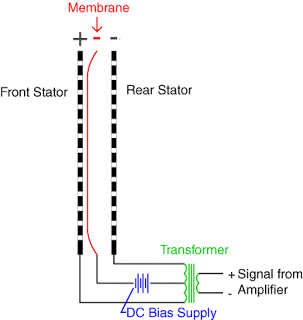
\includegraphics[width=0.5\textwidth]{images/esl_animation.png}
    \caption{Electrical concept}
    \label{f:intro:e-concept}
\end{figure}

The basic electrical concept of a electrostatic headphone can be seen in Fig. \ref{f:intro:e-concept}. An amplifier provides an input signal that is then transformed to yield the desired output voltage that drives the two stators. Additionally, there is a negative DC current that keeps the diaphragm charged.

\section{Required tools}
\label{s:tools}

\section{Required materials}
\label{s:materials}
\url{http://www.head-fi.org/t/826032/electrostatic-ear-speaker-diyers-suppliers-list}-> Suppliers list
\begin{enumerate}
    \item 1 mm PCB FR-4 and not laminate (for stators and dust protection spacers)
    \item 0.5 mm (or 0.6 mm) PCB (for spacers)
    \item 3 $\mu m$ Mylar (for diaphragm)
    \item 1-2 $\mu m$ Mylar (for dust protection, 1 $\mu m$ too thin maybe as very fragile) %AM-TODO
    \item \ldots (for coating the diaphragm) %AM-TODO
    \item Acrylic spray for insulating the stators
    \item Sheep skin leather (headband and pads)
    \item Wood (enclosure)
    \item Metal rods (headband)
    \item Foam (pads and headband)
\end{enumerate}

\url{http://www.ebay.com/itm/Electrostatic-Speaker-Membrane-Dupont-Mylar-C-3um-40M-/172275024448?_trksid=p2141725.m3641.l6368&rmvSB=true} -> Mylar source

For the amplifier:
\begin{enumerate}
    \item TODO
\end{enumerate}

\section{Building the driver}
\label{s:driver}

\subsection{Design of the stators and spacers}
\label{s:driver:design}
Diameter of the holes (2mm) should not be larger than the distance from stator to spacer. The holes in the stator should not cover the whole stator. Instead there should be a perimeter that acts as an air damper and avoids resonance frequencies in the upper midrange or lower treble. The size of the diaphragm is quite important as low frequencies require a large diaphragm surface. The active area should have a diameter of about 80 mm. The ratio of spacer thickness to diaphragm width should not be larger than 1:120 to avoid contact between stator and diaphragm. Lowering the bias voltage can help with very large ratios. Open area of the stators should be around 40\% in order to avoid issues with stability of the stator.

When drilling holes on the stator the feed rate should be at around 3600 mm/min.  For routing and cutting, it should be slowed down to around 1800 - 2400 mm/min.

In order to protect the diaphragm a dust and sweat protection needs to be used. This dust cover will be made from crumpled Mylar and will be located on the same side as the coating of diaphragm.

\url{http://www.head-fi.org/t/498292/my-diy-electrostatic-headphones/660#post_8897170} -> Design pictures of the Orpheus clones; apparently this design lacks some bass punch, maybe increase non-holed perimeter for improvements? Later on it is proposed to decrease the width a bit to improve stability. This would yield the dimensions of 110 x 74 mm (open area of 104 x 74 mm of orpheus clone).

\url{http://www.head-fi.org/t/498292/my-diy-electrostatic-headphones/1155#post_10142154} -> potential improvement of stability by making a hole in the center of the stators (one additional advantage: it's easier to detect issues with the diaphragm as it can be examined visually)

The edges of the spacers need to be sanded down a bit in order to avoid copper dust on the sides and spurious electrical contacts. Holes should be de-burred from copper.

\subsubsection{Gcode creation}
\label{s:driver:design:gcode}
In Linux Heekscnc can be used to create the gcode. Salome to do the CAD design. Inner ellipse: 55 x 37, outer: 65 x 47. Radius of holes: 1mm, multiplicator: 39 in x and 26 in y direction with distance 0.8421 and 0.88 in those directions, respectively.

Current setup:

\begin{itemize}
    \item FreeCad to make the designs -> export as svg
    \item Inkscape to place the svgs correctly \& create stator holes -> export as svg
    \item Makercam.com to create gcode.
\end{itemize}

CNC Drills:

\begin{itemize}
    \item 2mm drill for pcb
    \item 2mm end mill for pcb (coated)
    \item 6mm drill for wood 2-flute
    \item 2mm drill for wood 2-flute
\end{itemize}

Ordered via cnc-plus.de and sortec.de

\subsection{Etching the stators}
\label{s:driver:etching}
Etching the PCB board ensures that electrical contacts are only where they absolutely need to be. Furthermore, having less copper surface will result in a reduced capacitance and they will be easier to drive because of that. Toner transfer can be used to define the areas that should not be etched. After etching the stators can be protected by spraying thin layers of Acrylic paint on the copper (flat not glossy paint). This insulation avoids degradation of the copper surface and potential shorts when dust is present between the diaphragm and the stators. A small area needs to be left open so that wires can be soldered onto the stators.

\url{https://www.youtube.com/watch?v=jvCfgyWIpLI} -> youtube video to explain etching (3 parts)

\subsection{Tensioning the Mylar diaphragm}
\label{s:driver:tension}
Mylar with 3 $\mu m$ thickness is used to create the diaphragm. Thinner Mylar will cause a lack of bass, while thicker one will cause problem in treble and mids. The tensioning should be high enough as otherwise the diaphragm will collapse onto a stator but also low enough in order to not reduced the bass.
Different ways of tensioning the Mylar:
\begin{enumerate}
    \item With weights on the side
    \item Using a bicycle tire and inflating it
    \item Using tape to stretch it
\end{enumerate}
\begin{figure}[htb]
    \centering
    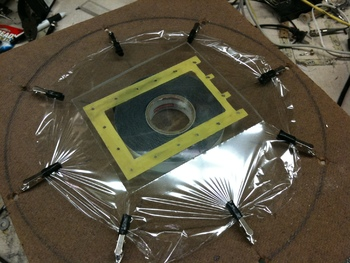
\includegraphics[width=0.5\textwidth]{images/mylar-tension-weight.png}
    \caption{A Mylar tensioning rig using weights}
    \label{f:driver:tension:weight}
\end{figure}
\begin{figure}[htb]
    \centering
    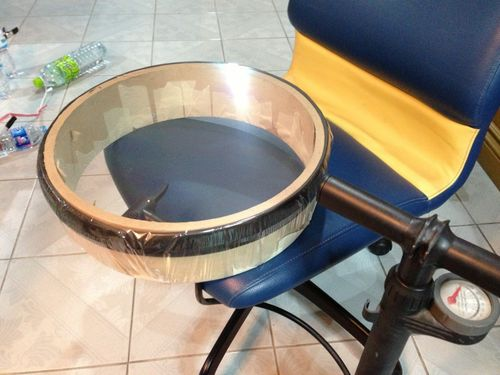
\includegraphics[width=0.5\textwidth]{images/mylar-tension-tire.png}
    \caption{A Mylar tensioning rig using an inflatable tire}
    \label{f:driver:tension:tire}
\end{figure}
\url{http://www.head-fi.org/t/498292/my-diy-electrostatic-headphones/720#post_9217468} -> Orpheus clone tensioning; weights should be larger between 0.8 and 1.0 kg. Preferred option

\url{http://www.head-fi.org/t/498292/my-diy-electrostatic-headphones/1095#post_9907534} -> tire tensioning jig.

Before putting it on the glass (and before coating) clean it with Acetone. To cut the Mylar after glueing use a soldering iron. Ensure there is no Mylar beyond the edges. The stators might warp slightly but this should be ok when assembling the driver.

Make sure the diaphragm is very well glued to the stator. The contact cement is applied to the spacer which is allowed to sit for 3-5 minutes. After that the spacer is put on the Mylar and a bond will be created immediately. A good contact can be achieved by running the finger along the spacers several times so that the glue is everywhere in contact with the spacer. See \url{http://www.head-fi.org/t/498292/my-diy-electrostatic-headphones/1215#post_10400583}

After glueing the Mylar onto the spacers knock them on the side of a table to check that the sound of both diaphragms is similar. If not, a hot air gun can be used to tension the one with a looser sound.

Tension is sufficient if wrinkles on the Mylar vanish during the procedure, corresponding to about 0.5\% of displacement. The two diaphragms need to be glued on the same mylar film so that the tension is the same on both sides.

\url{http://www.head-fi.org/t/498292/my-diy-electrostatic-headphones/1770#post_11440100} idea on how to identify the correct tension of the diaphragm by checking the free-air resonance frequency (should be between 100 and 200 Hz) using a white noise generator on one side and a microphone on the other.

\subsection{Coating the diaphragm}
As Mylar is not conductive an additional coating is required so that it can be charged. It basically should act as if it was a capacitor, so a coating that is conductive and has a high resistivity is ideal. Coating agents are:
\begin{enumerate}
    \item Staticide 6300 (anti static cleaner for monitors)
    \item Licron antistatic spray
    \item Swash Floor cleaner
\end{enumerate}
Coating is achieved by applying a small drop of Staticide onto the diaphragm and then spreading it with a sponge or microfibre cloth (lint free!). After it dries clean wipe the surface again with a dry lint free cloth.

Thread about coating: \url{http://www.diyaudio.com/forums/planars-exotics/109789-esl-diaphragm-coating.html}

Is this Staticide a gel?

\subsection{Assembly}
\label{s:driver:assembly}
Synthetic rubber glue (contact cement, UHU POR?, UHU Kontakt Kraftkleber fl\"ussig) is used to glue the diaphragm to the spacers. The dust protection screen must also be placed on some spacers (1mm thickness PCB) and must not be in contact with the stators. 2 $\mu m$ Mylar is crumpled and then stretched somewhat so that it doesn't touch the stators when on the spacer. This yields an ideal acoustically transparent material for dust protection. Normally, no dust cover is used on the outside. As no sweat protection is required on this side a very fine cloth could be used if needed. Only one spacer is glued to the diaphragm. This spacer will be the one facing the outside. The spacer on the inside will have the copper side in contact with the coated diaphragm and will be the one with the electrical contact to the DC bias voltage.
\begin{figure}[htb]
    \centering
    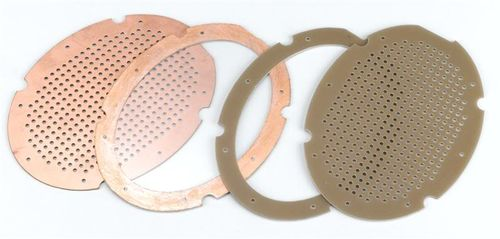
\includegraphics[width=0.5\textwidth]{images/arrangement.png}
    \caption{Arrangement and orientation of stators and spacers (missing the dust protection spacer and film)}
    \label{f:driver:assembly:arrangement}
\end{figure}

Plastic screws are used to assemble the driver unit.

Adhesive tape (masking tape) and pressurized air can be used to clean the dust of the diaphragm and stators. A magnifying glass should be used for checking cleanliness.

The driver can be tested by hooking it up to the amp and leave it as is for 3 to 4 hours without playing any music. The diaphragm should not be sucked to one side during this.

\subsection{TODO}
\begin{enumerate}
    \item What does it mean to bias the headphone for a certain voltage?
    \item What is used to coat the diaphragm? Coating is done with a wet sponge maybe.
    \item How much does the Mylar need to be stretched ($< 1\%$)? About 0.5 \% seems reasonable
    \item How to do accurate etching and what chemicals should be used? FeCl or HCl are options
    \item How can the surface resistance of the diaphragm be measures? Simply measure at opposite sides? Check multimeter capabilities as it might not be able to measure resistance in the GOhm range. Try to find alternative ways of measuring resistance if that is the case. Resistance should be around 10 - 100 MOhm per square (cm ?). \url{https://dannyelectronics.wordpress.com/2016/01/28/the-nano-ammeter-you-already-have/} shows a way to measure small currents
\end{enumerate}

\subsection{Potential improvements}
\begin{enumerate}
    \item Drill holes with two different sizes to get a larger hole to surface area ratio
    \item A space filling curve could be used to further reduce the copper on the stators
\end{enumerate}

\section{Building the enclosure}
\label{s:enclosure}
Wooden enclosures are potentially problematic as they can attract moisture which can cause electrical leakage. Sennheiser uses varnish on the outside of their wooden cups but none on the inside. It is possible to use a plastic O-ring to avoid direct contact between the wood and the driver.

\section{Building the headband}
\label{s:headband}

\url{http://www.head-fi.org/t/498292/my-diy-electrostatic-headphones/675#post_8943826}

Headband can be made out of a metal ruler and then covered with leather \url{http://www.head-fi.org/t/498292/my-diy-electrostatic-headphones/2385#post_13037825}.

\section{Building the earpads}
The earpads should be thick enough so that the bass is powerful and deep enough.
\label{s:pads}
\subsection{Potential improvements}
\begin{enumerate}
    \item Material should be leather on the inside. Sennheiser HE60/90 has fabric in contact with head, leather everywhere else. This makes it more comfortable
    \item It might be worth having harder foam on the inside as it will reduce resonances. Obviously this needs to be balanced to ensure comfort.
    \item Is it possible to make individual ear pads? Would allow for the use of harder materials. Moving your mouth changes the geometry so one would need to be careful.
\end{enumerate}
Post on ear pads: \url{http://www.head-fi.org/t/498292/my-diy-electrostatic-headphones/660#post_8930271}. Inner diameter of Orpheus earpads is 45mm x 90mm.

\section{Assembly}
\label{s:assembly}
Cables should be doubly insulated to withstand the high voltage. DIN plugs are used by many for electrostatic headphones but it might not be safe due to the high voltages, same for XLR. Ribbon cables rated for high voltages are recommended.

\subsection{TODO}
\begin{enumerate}
    \item Cable building (low capacitance)
    \item Connector building: need 6 pins ideally (3 for each side, for front and rear stator as well as one for the diaphragm DC voltage)
\end{enumerate}

\section{Amplifier}
\label{s:amp}
Due to the requirement of a continuously charged diaphragm and the high voltage requirements of the stators a dedicated amplifier is required for electrostatic headphones.
\begin{figure}[htb]
    \centering
    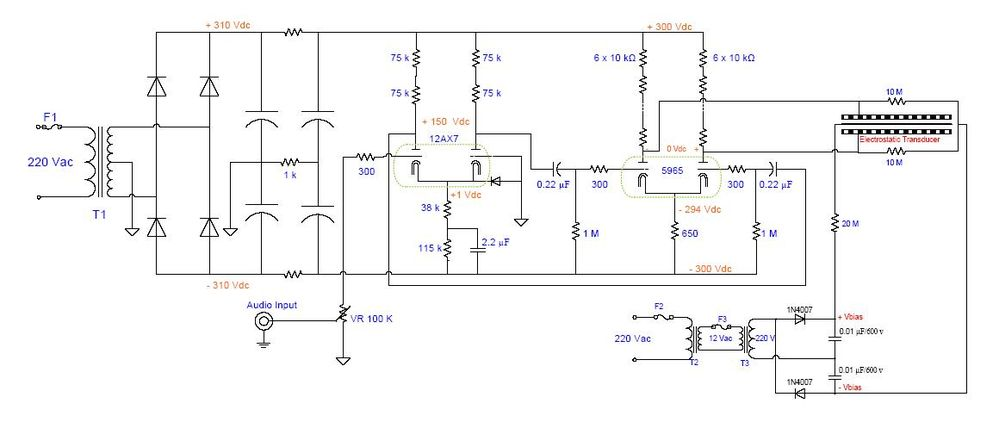
\includegraphics[width=0.5\textwidth]{images/wachara-amp.png}
    \caption{Amplifier design by Wachara C.}
    \label{f:amp:wachara}
\end{figure}
Discussion on this design: \url{http://www.head-fi.org/t/498292/my-diy-electrostatic-headphones/720#post_9182523}. Probably a step up transformer will be enough for starters

Other amplifier and transformer designs can be found here: \url{https://jazzman-esl-page.blogspot.co.at/2010/01/update-new-toroidal-step-up.html}

Check if it is possible to add a voltage regulator to try out different bias voltages easily \url{http://www.head-fi.org/t/498292/my-diy-electrostatic-headphones/1560#post_10959595}.

Amp safety: \url{http://www.head-fi.org/t/498292/my-diy-electrostatic-headphones/1455#post_10705917} and \url{http://www.head-fi.org/t/498292/my-diy-electrostatic-headphones/1470#post_10706261}

Check design in article \cite{ww_1979} and \cite{verwaal_2011}.

Turn ratio should be at least around 1:40.

\url{http://www.head-fi.org/t/498292/my-diy-electrostatic-headphones/2415#post_13059527} pdf with some links and amp designs

\section{Measurements}
\label{s:measurements}

Measurements with and without seal should be performed. The latter should give a peak at around 200 Hz which is the free-air resonance frequency. This frequency should be lower than 150 Hz for a good bass response.

\section{What to do different in the future}
\label{s:future}

\subsection{Closed headphones}
\label{s:future:closed}
Materials used for damping included felt, wool or other acoustically semi-transparent materials. Some also coat the inside of the enclosure with Bitumen.


\bibliographystyle{plain}
\bibliography{main}

\end{document}
